\chapter{附\texorpdfstring{\quad}{}录}
\renewcommand{\thesection}{{附录}\arabic{section}}
\setcounter{section}{0}
\section{zotero的设置}
\begin{figure}
	\centering
	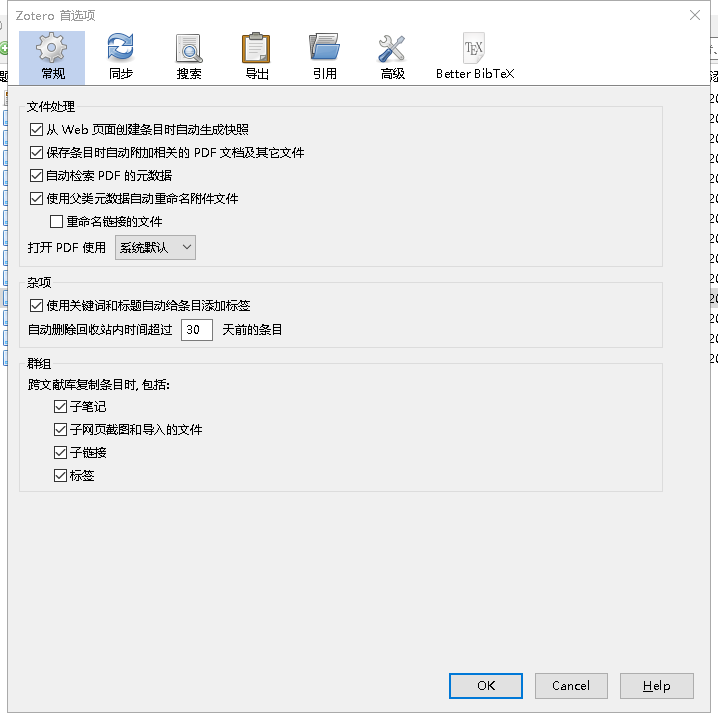
\includegraphics[scale=0.8]{Fig/zotero1.png}
	\caption{\label{op1}常规}
\end{figure}
\begin{figure}
	\centering
	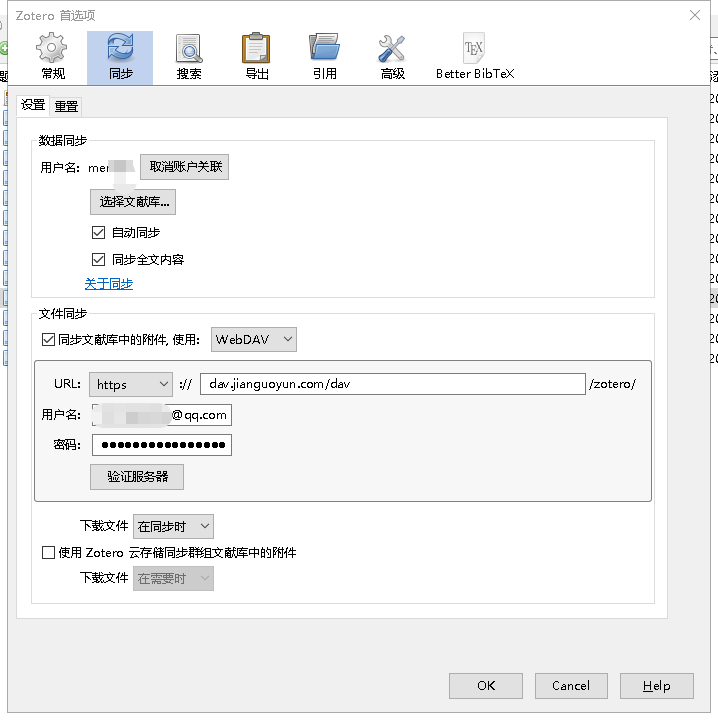
\includegraphics[scale=0.8]{Fig/zotero2.png}
	\caption{\label{op2}同步1}
\end{figure}
\begin{figure}
	\centering
	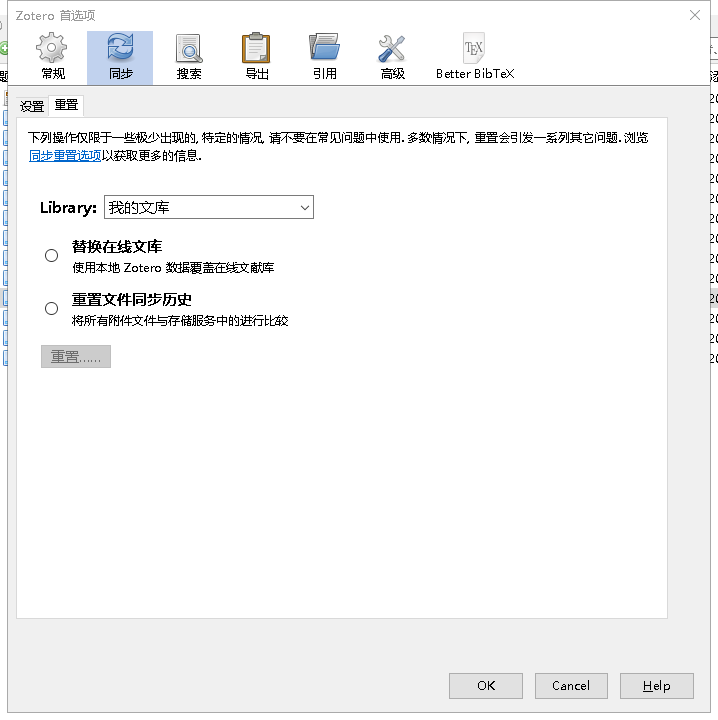
\includegraphics[scale=0.8]{Fig/zotero3.png}
	\caption{\label{op3}同步2}
\end{figure}
\begin{figure}
	\centering
	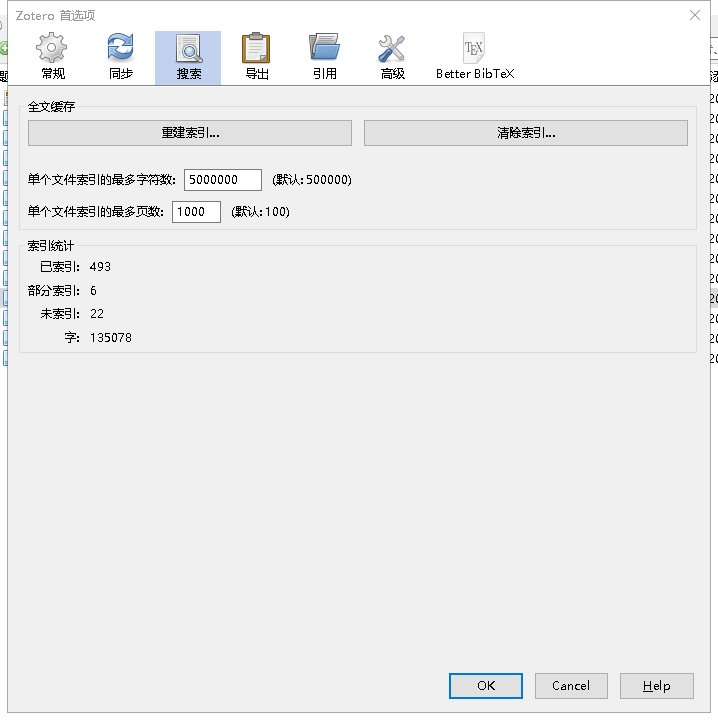
\includegraphics[scale=0.8]{Fig/zotero4.png}
	\caption{\label{op4}搜索}
\end{figure}
\begin{figure}
	\centering
	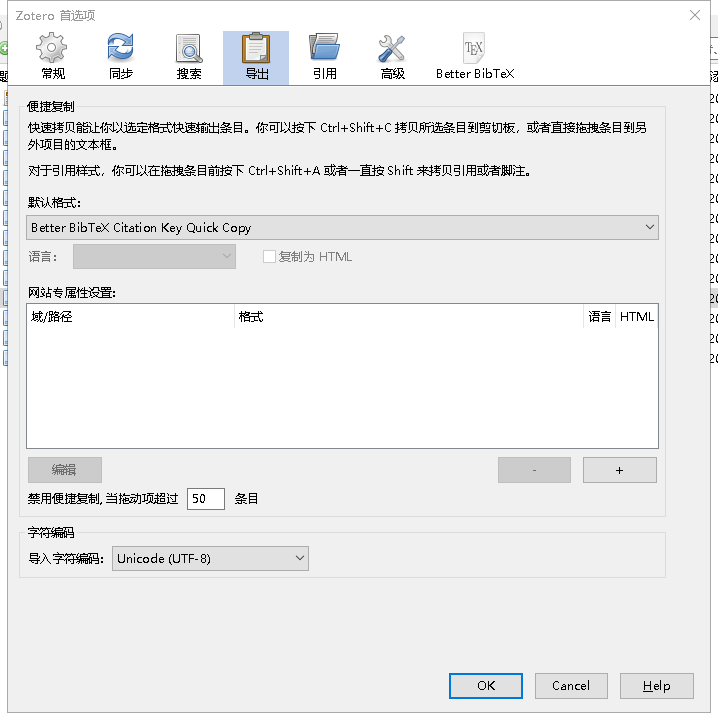
\includegraphics[scale=0.8]{Fig/zotero5.png}
	\caption{\label{op5}导出}
\end{figure}
\begin{figure}
	\centering
	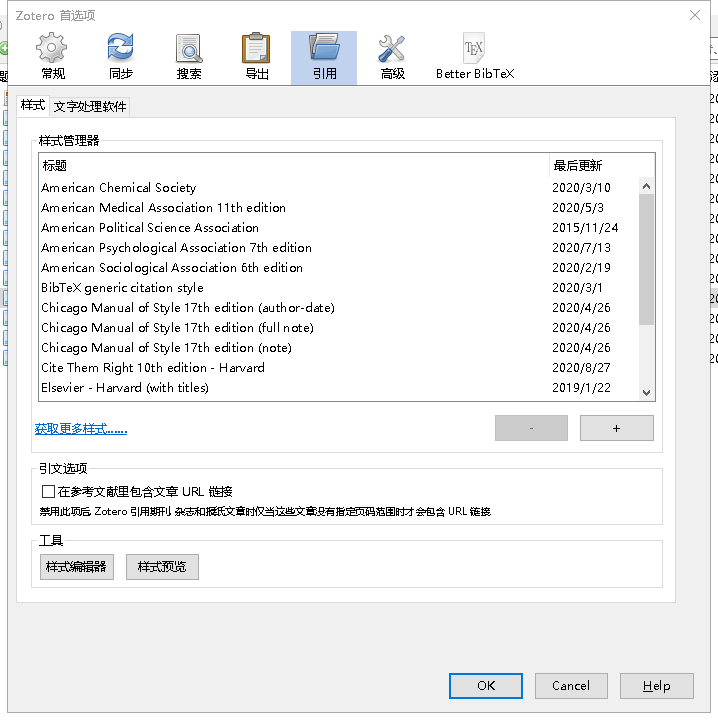
\includegraphics[scale=0.8]{Fig/zotero6.png}
	\caption{\label{op6}引用}
\end{figure}
\begin{figure}
	\centering
	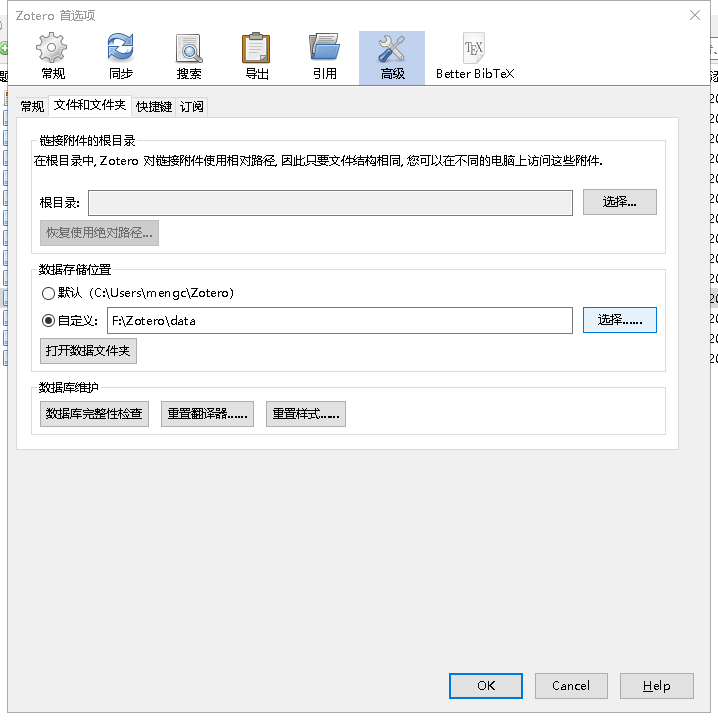
\includegraphics[scale=0.8]{Fig/zotero7.png}
	\caption{\label{op7}高级1}
\end{figure}
\begin{figure}
	\centering
	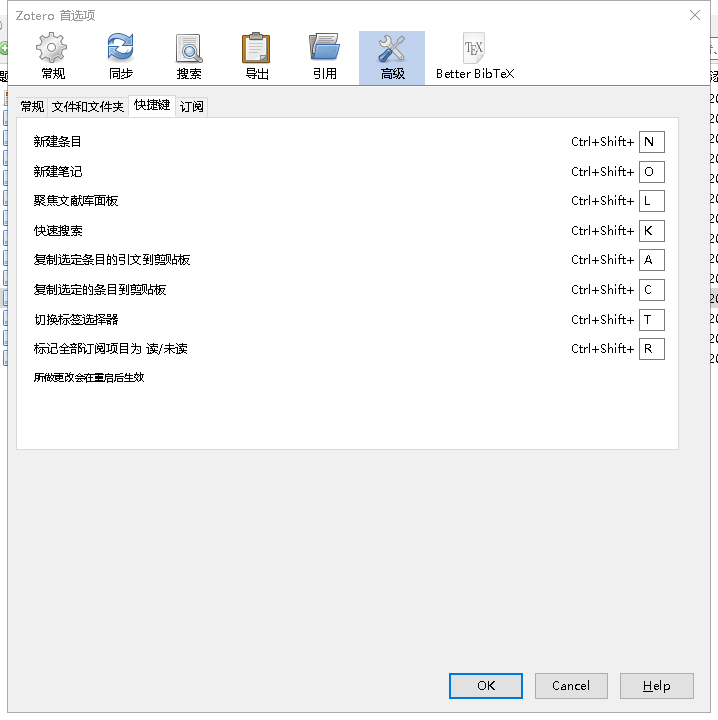
\includegraphics[scale=0.8]{Fig/zotero8.png}
	\caption{\label{op8}高级2}
\end{figure}
\begin{figure}
	\centering
	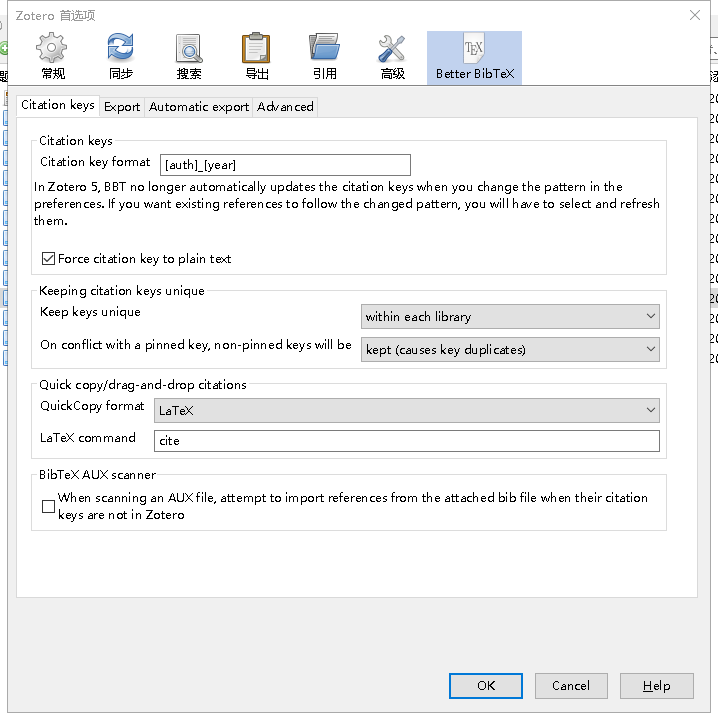
\includegraphics[scale=0.8]{Fig/zotero9.png}
	\caption{\label{op9}Better BibTeX1}
\end{figure}
\begin{figure}
	\centering
	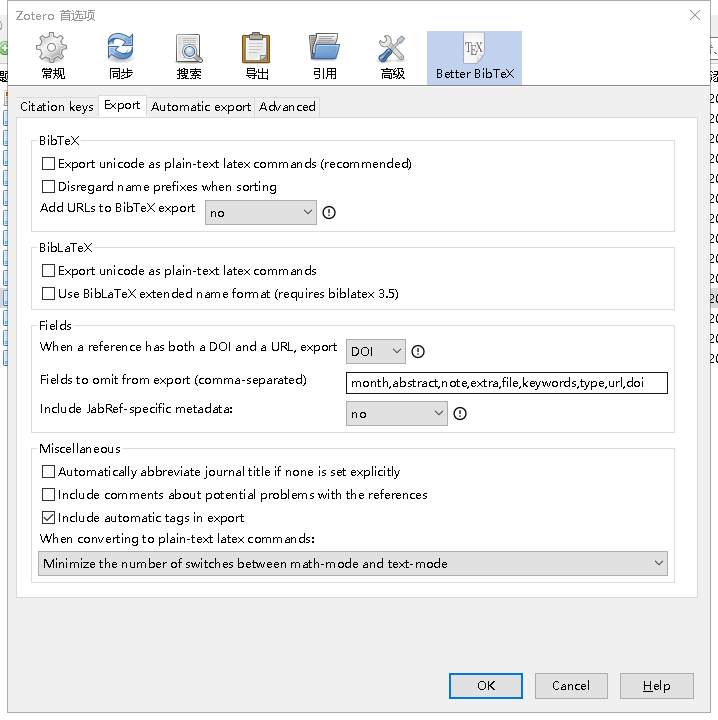
\includegraphics[scale=0.8]{Fig/zotero10.png}
	\caption{\label{op10}Better BibTeX2}
\end{figure}
\begin{figure}
	\centering
	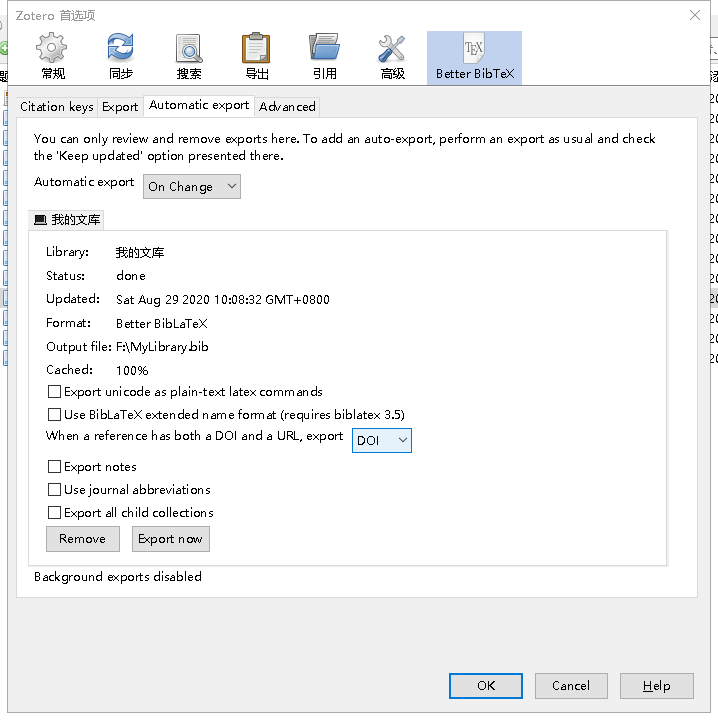
\includegraphics[scale=0.8]{Fig/zotero11.png}
	\caption{\label{op11}Better BibTeX3}
\end{figure}

\begin{figure}[htbp]
	\centering
	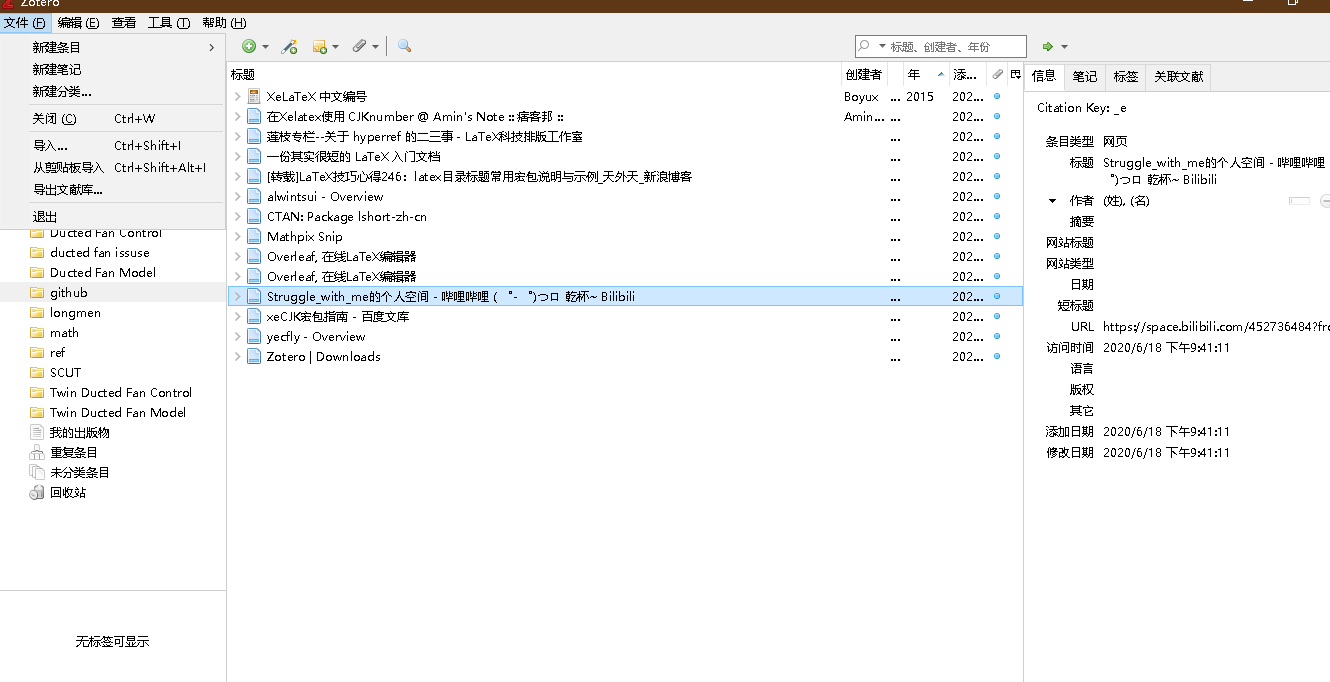
\includegraphics[scale=0.42]{Fig/zotero12.png}
	\caption{\label{output}导出文献库}
\end{figure}

\begin{figure}[htbp]
	\centering
	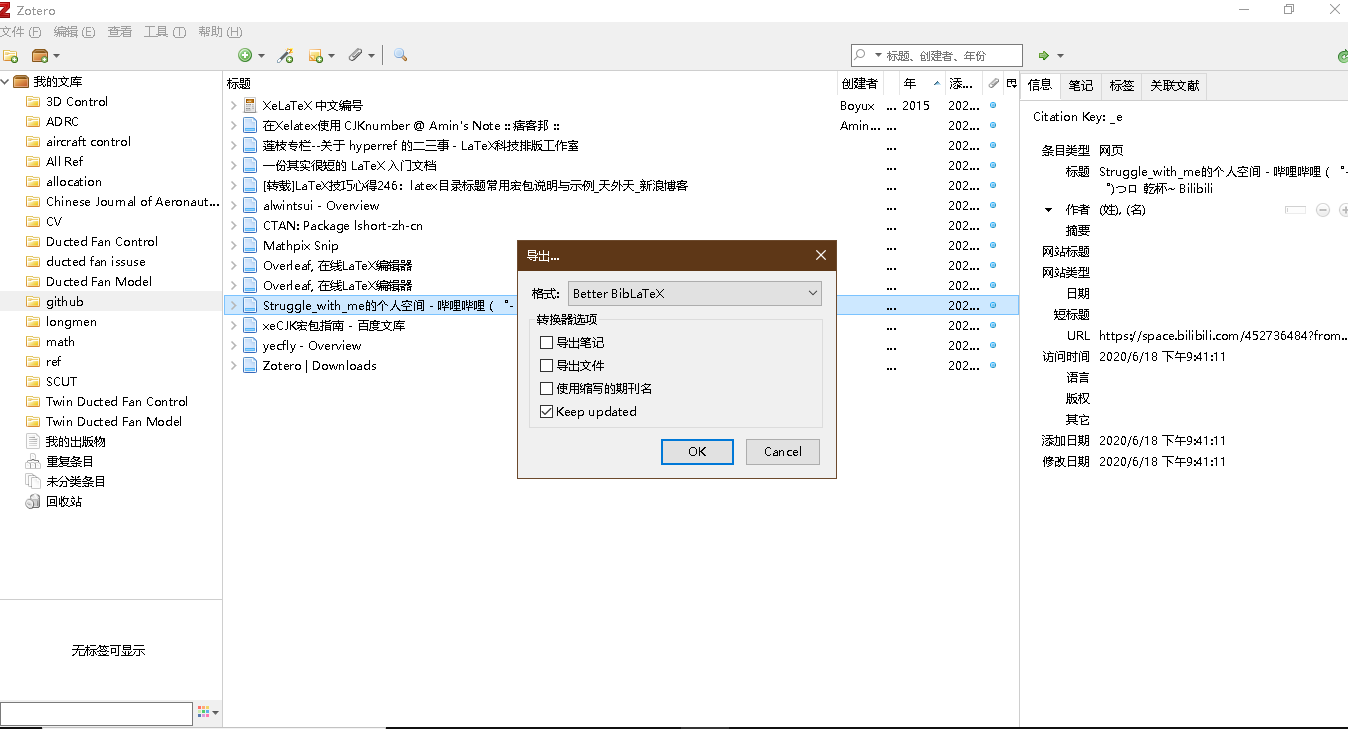
\includegraphics[scale=0.42]{Fig/zotero13.png}
	\caption{\label{output_format}导出格式}
\end{figure}

\begin{figure}[htbp]
	\centering
	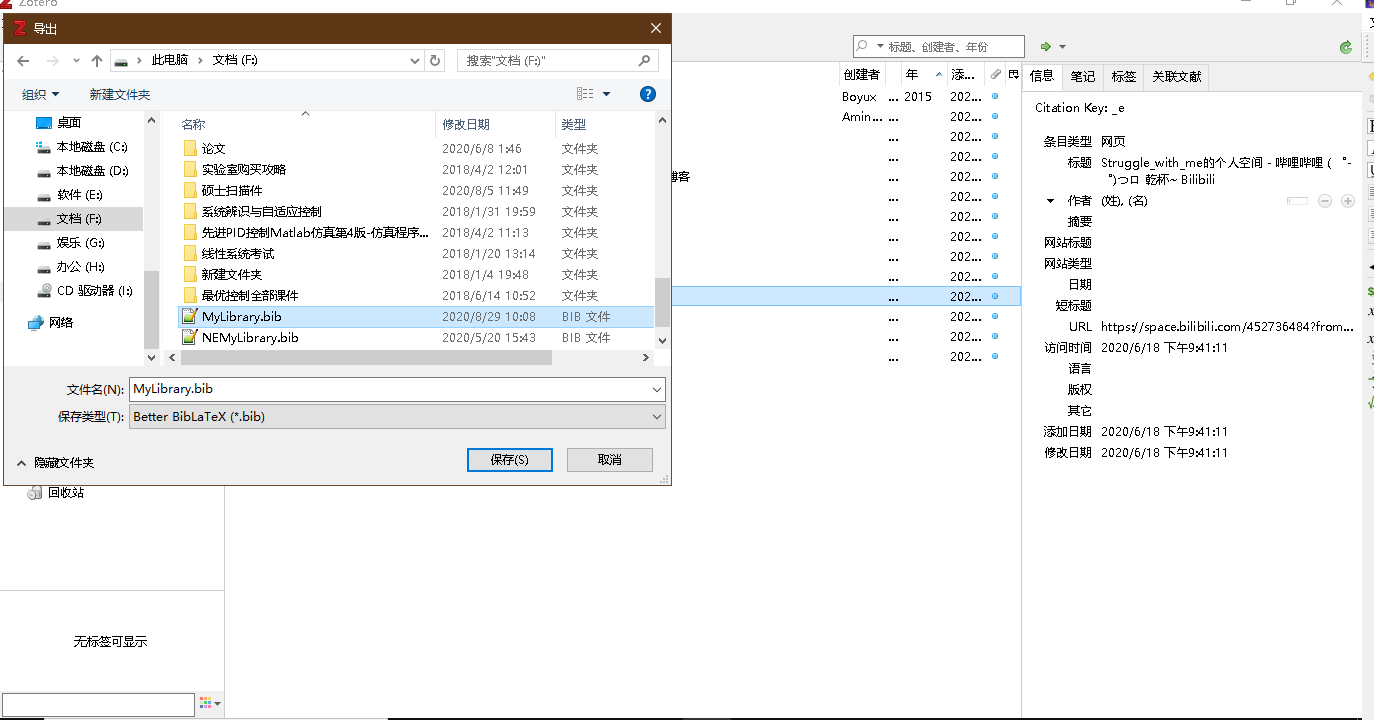
\includegraphics[scale=0.42]{Fig/zotero14.png}
	\caption{\label{output_name}导出文件名}
\end{figure}
\section{BibLatex}

